\documentclass{article}

\usepackage{mathpazo}
\usepackage{fontspec}
\usepackage{graphicx}
\usepackage{amsmath}
\usepackage{amssymb}
\usepackage{amsthm}
\usepackage{bm}
\usepackage{multirow}
\usepackage{hyperref}
\usepackage{braket}
\usepackage{bm}
\usepackage[perpage]{footmisc}
\usepackage[skip=0pt, width=0.75\textwidth, font=footnotesize]{caption}
\usepackage{todonotes}
\usepackage{listings}
\usepackage{siunitx}
\usepackage{tcolorbox}
\usepackage{booktabs}
\usepackage{algorithm}
\usepackage{algorithmic}
\usepackage[affil-it]{authblk}
\usepackage{ebgaramond}

\renewcommand*{\thefootnote}{\fnsymbol{footnote}}

\DeclareMathOperator{\Tr}{Tr}
\DeclareMathOperator{\Det}{Det}
\DeclareMathOperator{\Mod}{mod}
\renewcommand{\Re}{\operatorname{Re}}
\renewcommand{\Im}{\operatorname{Im}}

\theoremstyle{plain} \newtheorem{thm}{Theorem}[section]
\theoremstyle{definition} \newtheorem{df}{Definition}[section]
\theoremstyle{definition} \newtheorem{eg}{Example}
\theoremstyle{remark} \newtheorem*{rmk}{Remark}

% figures
\usepackage{import}
\usepackage{pdfpages}
\usepackage{xcolor}

\newcommand{\incfig}[2][]{%
  \def\svgwidth{{#1}\columnwidth}
    \import{./figures/}{#2.pdf_tex}
}

\title{The Monte Carlo Simulation of Ising Model}
\author{Yuanxing Duan}
\author{Shixin Hu}
\author{Fangyu Xiong}
\affil{School of Physics, Peking University}
\date{December 31, 2020}

\begin{document}
\maketitle

\abstract{Ising model is one of the most important models in the field of statistical mechanics. Despite its simplicity, it shows plenty of rich physics such as critical phenomena, and its relation to $\mathbb{Z}_2$ gauge theory. In this project, we use numerical Monte Carlo method, including the classical Metropolis and the so-called Worm algorithm to simulate the transverse field Ising model (TFI) in different spatial dimensions to reveal its critical behavior, such as its phase transition temperature, some critical exponents, as well as its critical dimension necessary to make the spontaneous symmetry breaking possible.}

\section{Introduction}
Ising model is one of the most fundamental model in statistical mechanics. The ferromagnetic transverse field Ising model Hamiltonian is:
\begin{equation}
	\mathcal{H}=-J\sum_{\langle ij\rangle}\sigma^z_i\sigma^z_j-h\sum_i\sigma_i^x
\end{equation}
where $\sigma_i^\alpha$ are the Pauli matrices representing the $\alpha$th component of the spin-1/2 on site $i$, and $J>0$. When $h=0$, corresponding to the classical Ising model, the eigenstates of this Hamiltonian are simply the direct product of the $\sigma^z$ basis of all sites, and we can simply replace the Pauli matrices $\sigma_i^z$ by their eigenvalues, which are either 1 or -1. When we turn on the transverse field $h$, quantum effects come in the story, since there will be fluctuations around the $\sigma^z$ basis of the classical Ising model and basically the true eigenstates of the quantum Ising model with finite $h$ will be an entangled state. 

One of the main aspects that make Ising model so important in statistical mechanics is its thermodynamic fluctuation, especially its behavior near criticality. For simplicity, we let $h=0$ and add a longitudinal field $h_z$ in the discussion of thermodynamic behavior, so the Hamiltonian becomes
\begin{equation}
	\mathcal{H}=-J\sum_{\langle ij\rangle}\sigma^z_i\sigma^z_j-h_z\sum_i\sigma_i^z.
\end{equation}
From statistical mechanics, we can easily write down its partition function, and use different methods to solve the problem (transfer matrix for dimension $d=1$, mean field for $d>1$, as well as various numerical methods). We take $d=2$ as an example to see its critical behavior. At first it has a finite critical temperature between paramagnetic phase at higher temperature and ferromagnetic phase at lower temperature:
\begin{gather}
	\sinh\left(\frac{2J}{T_c}\right)=1,\\
	T_c=\frac{2J}{\log(1+\sqrt{2})}.
\end{gather} 
The phase transition corresponds to a $\mathbb{Z}_2$ symmetry breaking. Next we can get different physical quantities with respect to temperature:
Magnetization:
\begin{equation}
	M=\langle\sigma_i^z\rangle\sim(T_c-T)^{\frac{1}{8}}.
\end{equation}
Susceptibility:
\begin{equation}
	\chi=\frac{\partial M}{\partial h_z}\sim(T-T_c)^{-\frac{7}{4}},
\end{equation}
and so on. 

In particular, the two-point correlation function $\Gamma(i-j)=\langle\sigma_i^z\sigma_j^z\rangle-\langle\sigma_i^z\rangle\langle\sigma_j^z\rangle$ behave differently at different temperature. When $T$ is away from $T_c$, the correlation function decay exponentially:
\begin{equation}
	\Gamma(i-j)\sim e^{\frac{|i-j|}{\xi(T)}},
\end{equation}
with correlation length $\xi(T)\sim\frac{1}{|T-T_c|}$. As $T\rightarrow T_c$, the correlation length diverges, and the correlation function behaves like
\begin{equation}
	\Gamma(i-j)\sim\frac{1}{|i-j|^{d-2+\eta}}.
\end{equation}
The critical exponents are listed as Table~\ref{tab:critical_exponents}.

\begin{table}[htpb]
  \centering
  \caption{Critical exponents of the Ising model.}
  \label{tab:critical_exponents}
  \begin{tabular}{crlc}
    \toprule
    Exponents & \multicolumn{2}{c}{Definition} & Ising Value \\
    $\alpha$ & $C$ & $ \propto (T-T_c)^{-\alpha}$ & 0 \\
    $\beta$ & $M$ & $ \propto (T_c-T)^\beta$ & 1/8 \\
    $\gamma$ & $\chi$ & $ \propto (T-T_c)^{-\gamma}$ & 7/4 \\
    $\delta$ & $M$ & $ \propto h^{1/\delta}$ & 15 \\
    \midrule
    $\nu$ & $\xi$ & $ \propto (T-T_c)^{-\nu}$ & 1 \\
    $\eta$ & $\varGamma(n)$ & $ \propto |n|^{2-d-\eta}$ & 1/4 \\
    \bottomrule
  \end{tabular}
\end{table}

Now let's see the case of quantum phase transition, where we turn on the transverse field $h$ and let $h_z=0$, so we go back to the original Hamiltonian. Taking $d=1$ as the example, we wish to get the partition function $\mathcal{Z}=\mathrm{Tr}[e^{-\beta H}]$. If we take $\beta=1/kT$ as imaginary time, we can calculate the partition function by path integral approach:
\begin{equation}
  \begin{aligned}
    \mathcal{Z}=\sum_{\left\lbrace S^z_{i,l}\right\rbrace }&\left\langle \left\lbrace S_{i,1}^z\right\rbrace\right|e^{-\Delta\tau H}\left|\left\lbrace S_{i,L}^z\right\rbrace\right\rangle\left\langle \left\lbrace S_{i,L}^z\right\rbrace\left|e^{-\Delta\tau H}\right|\left\lbrace S_{i,L-1}^z\right\rbrace\right\rangle \\
      &\times\cdots\left\langle \left\lbrace S_{i,2}^z\right\rbrace\left|e^{-\Delta\tau H}\right|\left\lbrace S_{i,1}^z\right\rbrace\right\rangle
  \end{aligned}
\end{equation}
where all $S^z_{i,l}$ are $\mathbb{Z}_2$ variables representing z-components of spins at site $i$ and time index $l$. The time slice $\Delta\tau=\beta/L$ and $L \to \infty$. After some calculation, we get the following partition function:
\begin{equation}
	\mathcal{Z}=\Lambda^{NL}\sum_{\left\lbrace S^z_{i,l}\right\rbrace }\exp\left[\sum_{i=1}^N\sum_{l=1}^L\left(\Delta\tau JS^z_{i,l}S^z_{i+1,l}+\gamma S^z_{i,l}S^z_{i,l+1}\right)\right]
\end{equation}
with $\gamma=-\frac{1}{2}\log[ \tanh(\Delta\tau h) ]$ and $\Lambda^2=\sinh(\Delta\tau h)\cosh(\Delta\tau h)$. So we can see that the 1+1 dimensional quantum Ising model is mapped to a 2+1 dimensional classical Ising model. Moreover, when we vary the transverse field $h$, the system will exhibit quantum phase transition.

\section{Worm Algorithm}
The Hamiltonian of quantum transverse-field Ising model (TFI) can be rewritten as
\begin{equation}
  \mathcal{H} = -t\sum_{\braket{ij}}\sigma_i^x\sigma_j^x - h\sum_{i}\sigma_i^z = K+U.
\end{equation}
And the interaction term $K$ can be further expressed in terms of the raising and lowering operators as
\begin{equation}
  K = K_1+K_2 = -t\sum_{\braket{ij}}(\sigma_i^+\sigma_j^-+\text{h.c.})-t\sum_{\braket{ij}}(\sigma_i^+\sigma_j^++\text{h.c.}).
\end{equation}
Then with the Holstein-Primakoff transformation $b_i(b_i^\dag) = \sigma_i^+(\sigma_i^-)$ and $n_i = b_i^\dag b_i = (\sigma_i^z+1)/2$, the TFI can be mapped onto a Bose-Hubbard (BH) model whose Hamiltonian is
\begin{equation}
  \mathcal{H} = -t\sum_{\braket{ij}}(b_i^\dag b_j+\text{h.c.})-t\sum_{\braket{ij}}(b_i^\dag b_j^\dag+\text{h.c.})-\mu\sum_{i}n_i, 
\end{equation}
where the chemical potential $\mu = 2h$. For this BH model, $K_1$ accounts for the hopping of a particle, and $K_2$ simultaneously creates or deletes a pair of nearest neighbouring (NN) particles.

We can use the imaginary-time path integral to represent the partition function: 
\begin{align}
  \mathcal{Z} &= \Tr \left(\mathrm{e}^{-\beta \mathcal{H}}\right) = \sum_{a_0}\bra{\alpha_0}\mathrm{e}^{-\beta \mathcal{H}}\ket{\alpha_0}\\
              &= \lim_{\mathrm{d}\tau = \frac{\beta}{n}, n \to \infty} \sum_{\{\alpha_i\}}\bra{\alpha_0}\mathrm{e}^{-\mathcal{H}\mathrm{d}\tau}\ket{\alpha_{n-1}}\cdots \bra{\alpha_i}\mathrm{e}^{-\mathcal{H}\mathrm{d}\tau}\ket{\alpha_0}\\
              &= \sum_{\alpha_0}\sum_{\mathcal{N}}^{\infty}\int_{0}^{\beta}\int_{\tau_1}^{\beta}\cdots \int_{\tau_{\mathcal{N}-1}}^{\beta} \prod_{k=1}^{\mathcal{N}}\mathrm{d}\tau_k\,F(t, h),
\end{align}
with the integrand function
\begin{equation}
  F(t, h) = t^{\mathcal{N}_h+\mathcal{N}_p}\mathrm{e}^{-\int_{0}^{\beta}U(\tau)\,\mathrm{d}\tau},
  \label{eq:integrand}
\end{equation}
where $\mathcal{N}_h$ and $\mathcal{N}_p$ are the number of hopping and pairing kinks. So the partition function $\mathcal{Z}$ can be regarded as the summation of different configuration in the $(d+1)$D space-time, of which the statistical probability is
\begin{equation}
  W_{\mathcal{Z}}(t, h) = \prod_{k=1}^{\mathcal{N}}\mathrm{d}\tau\,F(t, h).
\end{equation}

In this representation, each configuration can be viewed in the following way. For each lattice site $i$, the spin $\sigma_i^z$ may be flipped by the hopping or pairing at some imaginary time $\tau_k$. Since either hopping or pairing term simultaneously flips spins at two NN sites, so one can construct a loop by following the spin-up segments along the imaginary time, and kinks which labels the spin flips of two NN sites. Hence, a configuration can be identified with several loops of spin-up in the $(d+1)$D space-time.

Then, we can extend the configuration space $\mathcal{Z}$ to $\mathcal{G}$ by including two defects, which corresponds to the spin-spin correlation function:
\begin{equation}
  \mathcal{G}(\bm{x}_I, \tau_I; \bm{x}_M, \tau_M) = \Tr\left[ T_\tau\left( \sigma_I^x(\tau_I)\sigma_M^x(\tau_M)\mathrm{e}^{-\beta\mathcal{H}} \right) \right],
\end{equation}
where $T_\tau$ is the $\tau$-ordering operator. In the configuration space $\mathcal{G}$, each configuration can be viewed as several loops and an open path with two ending points ``Ira'' ($I$) and ``Masha'' ($M$), which correspond to the two spins in the correlation function. Similarly, the statistical weight of the $\mathcal{G}$ configuration can be written as
\begin{equation}
  W_\mathcal{G} = \frac{\mathrm{d}\tau_I\mathrm{d}\tau_M}{\omega_G} \prod_{k=1}^{\mathcal{N}}\mathrm{d}\tau_k\,F(t, h),
\end{equation}
here $\omega_G$ is an arbitrary positive number. And when $I$ coincides with $M$, the open path forms a loop, the configuration in the $\mathcal{G}$ space turns into one in the $\mathcal{Z}$ space.

The key idea of the worm algorithm is to move the defects $I$ and $M$ of the open path (like a worm wriggling) to produce different $\mathcal{G}$ and $\mathcal{Z}$ configurations for sampling. For ergodicity, the simulation should be able to change the number of kinks, the space-time location of kinks, and that of the defects $I$ and $M$. So we perform the following three kinds of updates:
\begin{figure}[htpb]
  \centering
  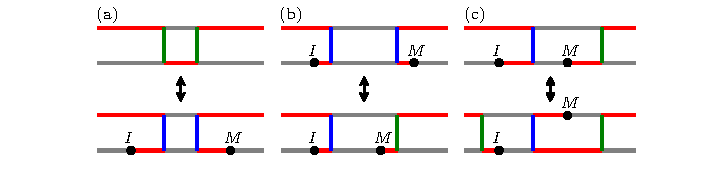
\includegraphics[width=\textwidth]{figs/updates.pdf}
  \caption{Three different kinds of updates. The red (gray) line denotes spin-up (spin-down) states, and the green (blue) line denotes hopping (pairing) kinks. (a) Create/annihilate defects $I$ and $M$. (b) Move imaginary time of defect $M$. (c) Insert/delete a kink.}
  \label{fig:updates}
\end{figure}
\begin{enumerate}
  \item \textit{Create/annihilate defects $I$ and $M$.}
    If the current configuration is in the $\mathcal{Z}$ space, then ``creating defects'' is the only possible update. We randomly picks up a point $(\bm{x}_I, \tau_I)$ in the whole space-time, draws a uniformly distributed time displacement $\delta \in [-\tau_a/2, \tau/2]$ and $\delta \ne 0$, assigns $\bm{x}_M = \bm{x}_I$ and $\tau_M = \Mod(\tau_I+\delta, \beta)$, and flips the spin state between $I$ and $M$.

    The reverse operation of ``creating defects'' is ``annihilating defects'', which is chosen with an \textit{a priori} probability $\mathcal{A}_a$ in the $\mathcal{G}$ space. By annihilating defects $I$ and $M$ and flipping the spin state in-between, a $\mathcal{G}$ configuration are changed into a $\mathcal{Z}$ configuration. The annihilation is possible only if $I$ and $M$ are on the same world line $\bm{x}_I = \bm{x}_M$ and their imaginary-time displacement $\min\{|\tau_I-\tau_M|, \beta-|\tau_I-\tau_M|\} \le \tau_a/2$.

    The detailed-balance condition of creating and annihilating defects reads as
    \begin{equation}
      \frac{\mathrm{d}\tau_I}{\beta N}\frac{\mathrm{d}\tau_M}{\tau_a}\cdot W_\mathcal{Z}\cdot\mathcal{P}_\text{crea} = \mathcal{A}_a\cdot W_\mathcal{G}\cdot\mathcal{P}_\text{anni},
    \end{equation}
    which leads to the acceptance probabilities
    \begin{gather}
      P_\text{crea} = \min \left[ 1, \mathcal{A}_a \tau_a \frac{\beta N}{\omega_G}\frac{F_\text{new}}{F_\text{old}} \right],\\
      P_\text{anni} = \min\left[ 1, \frac{1}{\mathcal{A}_a \tau_a}\frac{\omega_G}{\beta N}\frac{F_\text{new}}{F_\text{old}} \right],
    \end{gather}
    where $F_\text{old}$ and $F_\text{new}$ are given by Eq.~\ref{eq:integrand}. And here we choose $\omega = \beta N$ to make the calculation simpler.

  \item \textit{Move imaginary time of defect $M$.}
    This kind of update is chosen with a probability $\mathcal{A}_b$ in the $\mathcal{G}$ space. We randomly select a imaginary-time displacement $\delta \in [-\tau_b/2, \tau_b/2]$ and $\delta\ne 0$, assigns $\tau'_M = \Mod(\tau_M+\delta,\beta)$ for the new temporal location of defect $M$, and flips the spin states in-between. The acceptance probability is
    \begin{equation}
      P_\text{move} = \min\left\{1, \frac{F_\text{new}}{F_\text{old}}\right\}.
    \end{equation}

  \item \textit{Insert/delete a kink.}
    Each operation is chosen with a probability $\mathcal{A}_c$ in the $\mathcal{G}$ space. When ``inserting a kink'', we randomly choose one of the $z_d = 2d$ neighbouring world lines of $\bm{x}_M$, denote it as $\bm{x}_M'$, and updates the location of $M$ from $(\bm{x}_M, \tau_M)$ to $(\bm{x}_M', \tau_M)$. Meanwhile, we insert a kink $k$ between world lines ${\mathbf x}_M$ and ${\mathbf x}'_M$ at imaginary time $\tau_k = \Mod(\tau_M+\delta,\beta)$, with a random displacement $\delta \in [-\tau_c/2, \tau_c/2]$ and $\delta\neq 0$. Further, the spin states between $\tau_M$ and $\tau_k$, on both ${\mathbf x}_M$ and ${\mathbf x}'_M$, are flipped.

    In the reverse operation, ``deleting a kink'', we also pick up a random neighbouring world line ${\mathbf x}'_M$ of $\mathbf{x}_M$ and moves $M$ from $({\mathbf x}_M, \tau_M)$ to $({\mathbf x}'_M, \tau_M)$. If there is no kink that connects world lines ${\mathbf x}_M$ and ${\mathbf x}'_M$ in the imaginary-time domain $[\tau_M-\tau_c/2, \tau_M+\tau_c/2]$, the operation is rejected. Otherwise, we randomly pick up one of those  $n_k$ in this region and delete it, and meanwhile flip the spin states on both world lines between $\tau_M$ and the imaginary time of the deleted kink.

    The detailed balance condition of this pair of operations is
    \begin{equation}
      \mathcal{A}_c\cdot\frac{1}{z_d}\cdot\frac{\mathrm{d}\tau}{\tau_c}\cdot W\cdot \mathcal{P}_\text{inse} = \mathcal{A}_c\cdot\frac{1}{z_d}\cdot\frac{1}{n_k}\cdot W_+\cdot \mathcal{P}_\text{dele},
    \end{equation}
    which leads to the acceptance probabilities
    \begin{gather}
      P_\text{inse} = \min\left[1, \frac{\tau_c}{n_k+1}\frac{F_\text{new}}{F_\text{old}}\right],\\
      P_\text{dele} = \min\left[1, \frac{n_k}{\tau_c}\frac{F_\text{new}}{F_\text{old}}\right].
    \end{gather}
\end{enumerate}

The worm algorithm can be concluded as Algorithm~\ref{algorithm}, in which \textit{a priori} probabilities satisfy $\mathcal{A}_a+\mathcal{A}_b+2\mathcal{A}_c = 1$.\\
\begin{minipage}{\linewidth}
  \begin{algorithm}[H]
  \caption{Worm algorithm}
  \label{algorithm}
  \begin{algorithmic}
    \STATE initialization;
    \STATE thermalization;
    \LOOP
      \IF{it is a  $\mathcal{Z}$ configuration}
        \STATE compute statistical quantities of this configuration;
        \STATE choose the ``creating defects $(I, M)$'' operation;
      \ELSE
        \STATE  choose an operation with its \textit{a priori}  probability;
        except ``creating defects $(I, M)$'';
      \ENDIF
      \STATE calculate the acceptance probability $P$ and carry out the operation with the probability $P$;
    \ENDLOOP
  \end{algorithmic}
\end{algorithm}
\end{minipage}
\vspace{3mm}

\section{Numerical Results}
We calculate the phase transition of TFI based on the worm algorithm. When the transverse field $h = 0$, there exists the $\mathbb{Z}_2$ symmetry which means that the spin-up and spin-down states are fully balanced, and the system is in a ferromagnetic phase. As $h$ turns on, the system evolves into a disordered phase with the spin-down state being suppressed. And once $h > h_c$, the system enters into the spin-up ordered phase through a second-order quantum phase transition. Because it is $h_c/t$ rather than $h_c$ itself that describes the physical properties of the model, we simply set $t = 1$ for simplicity of calculation.

We discretize the imaginary time so that the calculation is more efficient, which makes our system is indeed a $(d+1)$D lattice. Because the dynamic critical exponent $z = 1$ for the TFI, we choose the inverse temperature $\beta = L$, where $L$ is the spatial lattice size. We also applied the periodic boundary conditions, so the space-time lattice is a torus in fact. We mainly calculate the 1D TFI with $L = 64$ and $128$ in our current work.

To get the critical point $h_c$, we focus on the topological properties instead of physical quantities like the magnetic susceptibility of $\mathcal{Z}$ configurations when sampling. In more detail, for a given $\mathcal{Z}$ configuration, we can count the winding number $W_i^l$ of the $l$-th loop along the $i$-th spatial direction. The total winding number $W_i = \sum_{l}W_i^l$ can be used to determine whether the $\mathcal{Z}$ configuration wrap along the $i$-th direction or not, which is indicated as $R_i = 1$ if $W_i > 0$ and $R_i = 0$ otherwise. Then the average wrapping probability $R = \sum_{i=1}\braket{R_i}/d$ is calculated, which indicates whether the in-site energy $U$ or the interaction $K$ dominates. If $|h| \gg 1$, $U$ dominates, which means that the loops are small and difficult to percolate, hence $R$ should be small (near $0$). But if $|h| \ll 1$, $K$ dominates, so $R$ should be large (near $1$). In calculation, we traverse all loops of a $\mathcal{Z}$ configurationo based on depth-first search (DFS).

\begin{figure}[htpb]
  \centering
  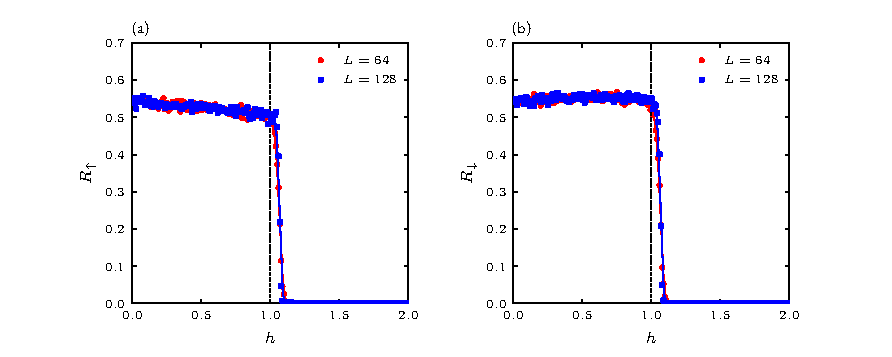
\includegraphics[width=\textwidth]{figs/wrapping_probability.pdf}
  \caption{Wrapping probability of spin-up $R$ versus the transverse field $h$.}
  \label{fig:wrapping_probability}
\end{figure}

The Monte Carlo results in Fig.~\ref{fig:wrapping_probability} show that the spin-up loops display critical behaviors near $h = h_c = 1$, which is the theoretical value of the critical point. When $h < h_c$, $R$ has non-zero values, which means the system is indeed in an interaction-dominating phase. When $h$ increases, $R$ slowly decreases, which is easy to understand, since the increasing $h$ makes $\mathcal{Z}$ configurations with ``longer fragments'' of spin-up states for a given lattice site along the imaginary time direction are more possible to be sampled, which slightly restrains the wrapping probability of spin-up. If $h$ increases further over $h_c$, $R$ will drop to $0$ quickly. This is because in this phase, most sampled $\mathcal{Z}$ configurations will be dominated by spin-up states, which makes the number of kinks too small for spin-up loops to percolate.
\end{document}
